\documentclass[conference]{IEEEtran}
\IEEEoverridecommandlockouts

\usepackage{cite}
\usepackage{amsmath,amssymb,amsfonts}
\usepackage{graphicx}
\usepackage{textcomp}
\usepackage{xcolor}
\usepackage{booktabs}
\usepackage{array}
\usepackage{tikz}
\usetikzlibrary{shapes,arrows,positioning,fit,calc,decorations.pathreplacing}
\usepackage{url}
\usepackage{microtype}
\usepackage{enumitem}
\usepackage{multirow}

\setlist[itemize]{leftmargin=*,itemsep=1pt,topsep=2pt}
\setlist[enumerate]{leftmargin=*,itemsep=1pt,topsep=2pt}

%-----------------------------------------------------------------------
\begin{document}

\title{TOBACCOGUARD: A SATELLITE-BASED TOBACCO CROP\\
HEALTH MONITORING SYSTEM USING MACHINE LEARNING}

\author{
  \IEEEauthorblockN{$^{1}$Prince Rupiya \quad $^{2}$Mr Manyonganise}\\[2pt]
  \IEEEauthorblockA{%
    $^{1}$\texttt{h220536m@hit.ac.zw} \quad
    }\\[2pt]
  Harare Institute of Technology, Harare, Zimbabwe\\
  Department of Information Technology, Harare Institute of Technology
}

\maketitle

%-----------------------------------------------------------------------
\begin{abstract}
Tobacco is a critical export crop for Zimbabwe, yet smallholder farmers
lack accessible tools for timely detection of crop stress. Manual scouting
is labour-intensive and is typically too infrequent to prevent yield loss.
This paper presents TobaccoGuard, a web-based platform that monitors
tobacco crop health by combining free satellite imagery from Google Earth
Engine (GEE) and the Copernicus Sentinel-2 archive with a machine
learning classification pipeline. Farmers register geo-referenced field
polygons on an interactive Leaflet map, after which the system
automatically retrieves a 90-day multi-temporal NDVI time series,
derives five agronomic features, and applies a multinomial logistic
regression classifier to assign one of three health statuses:
\textsc{healthy}, \textsc{moderate\_stress}, or \textsc{high\_stress}.
The classifier achieved 97\,\% overall accuracy on a held-out test set
of 122 samples, with per-class F1-scores of 0.99, 0.97, and 0.95
respectively. A rule-based recommendation engine translates classifier
outputs into four targeted agronomic interventions. The system is
implemented as a Next.js\,14 full-stack application with SQLite
persistence and executes ML inference natively in TypeScript at runtime,
eliminating any dependency on a Python interpreter in production.
Functional evaluation across eight end-to-end test scenarios confirmed
correct behaviour throughout the pipeline. The prototype demonstrates
that a deployable, zero-licensing-cost precision agriculture tool for
smallholder tobacco farmers is achievable using freely available
satellite and cloud infrastructure.
\end{abstract}

\begin{IEEEkeywords}
Normalized Difference Vegetation Index (NDVI), satellite remote sensing,
Google Earth Engine, tobacco crop monitoring, logistic regression,
Sentinel-2, precision agriculture, crop health classification, Zimbabwe
\end{IEEEkeywords}

%-----------------------------------------------------------------------
\section{Introduction}

Tobacco remains one of Zimbabwe's most significant agricultural export
commodities, contributing substantially to foreign currency earnings and
rural livelihoods \cite{zimstats2023}. The country's tobacco production
relies heavily on smallholder farmers, whose plots typically range from
0.5 to 5~hectares and whose access to technical support is constrained
by limited extension officer availability. These farmers currently rely
on visual field inspection and periodic advisory visits to identify crop
stress. This reactive approach means that water stress, nutrient
deficiency, and disease pressure are frequently detected only after
visible leaf wilting or discolouration has occurred, by which point
significant yield loss may already be irreversible \cite{xue2017}.

Satellite remote sensing offers a scalable alternative that operates
continuously and at near-zero marginal cost per additional field
monitored. The Normalized Difference Vegetation Index (NDVI), computed
from red and near-infrared reflectance bands as $(B8 - B4)/(B8 + B4)$,
provides an objective, non-invasive proxy for canopy photosynthetic
activity and has been validated as an early indicator of plant stress
across a wide range of crops before visual symptoms become apparent
\cite{rouse1974}. The Sentinel-2 satellite constellation, operated by
the European Space Agency under the Copernicus programme, delivers freely
accessible 10-metre-resolution multispectral imagery with an approximate
five-day revisit time, making regular field-level monitoring practical
without recurring data licensing costs \cite{drusch2012}.

Despite these opportunities, commercially available precision agriculture
platforms such as EOSDA Crop Monitoring and Cropio impose subscription
fees that are prohibitive for smallholder farmers or the institutions
that serve them. Open-source GIS tools such as QGIS and Google Earth
desktop exist but require significant remote sensing expertise to
operate, well beyond that of most extension officers or farmer
cooperatives. There is therefore a clear gap for a low-cost,
user-friendly, web-based monitoring tool tailored to the Zimbabwean
smallholder tobacco context.

This paper presents TobaccoGuard, a prototype system that addresses this
gap by integrating freely available satellite data retrieval,
domain-specific feature engineering, and a lightweight machine learning
classifier into a deployable web application. Our principal contributions
are:
\begin{enumerate}
  \item A full-stack satellite monitoring pipeline that retrieves and
    processes Sentinel-2 NDVI time series via the GEE API and derives
    agronomic features at field polygon granularity.
  \item A multinomial logistic regression classifier trained offline
    with scikit-learn and serialised to a JSON coefficient file, enabling
    native TypeScript inference with no Python dependency at runtime.
  \item A rule-based recommendation engine that maps classifier outputs
    and feature values to four targeted field management interventions.
  \item An end-to-end functional evaluation demonstrating correct
    pipeline behaviour across all eight test scenarios.
\end{enumerate}

The remainder of this paper is structured as follows. Section~II reviews
related work on NDVI-based crop monitoring and machine learning for
crop classification. Section~III presents the system design including
architecture, database model, and algorithm design. Section~IV details
the implementation. Section~V reports evaluation results. Section~VI
discusses findings and limitations. Section~VII concludes.

%-----------------------------------------------------------------------
\section{Literature Review}

Remote sensing applications in agriculture have expanded considerably
since the public release of large-scale satellite image archives. NDVI
computed from Landsat and MODIS imagery has been applied for decades to
estimate crop yield, biomass, and canopy cover \cite{xue2017}. The shift
to Sentinel-2's 10-metre spatial resolution has more recently enabled
monitoring at the level of individual smallholder fields, which was
previously impractical with 30-metre or 250-metre resolution data.

\subsection{NDVI-Based Crop Stress Detection}

Several studies have validated NDVI time series from Sentinel-2 for crop
stress detection. Delegido et al.\ demonstrated that multi-temporal NDVI
profiles can reliably differentiate between irrigated and rain-fed maize
fields at classification accuracies exceeding 90\,\%, showing that
trajectory shape rather than single-date index values carries most
discriminative information \cite{delegido2011}. Kussul et al.\ further
showed that incorporating temporal trend features derived from NDVI time
series substantially improves classification accuracy for smallholder
crop mapping in Sub-Saharan Africa, where phenological timing is more
variable than in large-scale mechanised farming systems
\cite{kussul2017}. These findings motivated the inclusion of NDVI slope
(trend) and variance as explicit features in the present work rather than
relying solely on the temporal mean.

Tobacco-specific remote sensing research remains limited compared to
staple grains, but the general relationship between NDVI and leaf
photosynthetic capacity is well-established across broad-leaved crop
species. Below NDVI~$\approx$~0.35, significant chlorophyll reduction
associated with water stress or nutrient deficiency is expected; above
NDVI~$\approx$~0.60, canopy closure is typically adequate and the crop
is unlikely to be in acute stress \cite{xue2017}.

\subsection{Machine Learning for Crop Classification}

Machine learning approaches to remote sensing crop health classification
span logistic regression, support vector machines, random forests, and
deep convolutional networks. Kpienbaareh et al.\ conducted a comparative
study of these classifiers for smallholder crop mapping in Ghana using
Sentinel-1 and Sentinel-2 features and found that logistic regression
achieved classification accuracy within 2\,\% of more complex ensemble
models when training sets contained fewer than 1\,000 labelled samples
and features were carefully engineered \cite{kpienbaareh2021}. This
result is consistent with the bias-variance tradeoff literature: with
limited training data, high-capacity models such as gradient boosted
trees tend to overfit, while a regularised linear classifier generalises
more reliably.

The practical case for logistic regression in this project was further
strengthened by the deployment constraint that ML inference must execute
natively in a Node.js TypeScript environment without a Python subprocess.
A logistic regression model reduces to a matrix-vector multiplication
followed by softmax normalisation, which is straightforward to implement
in any language from a serialised coefficient file. More complex models
such as random forests would require a significantly larger runtime
library (e.g., ONNX Runtime) and a more complex serialisation scheme.

\subsection{Existing Monitoring Platforms}

Table~\ref{tab:comparison} summarises commercially available and
prototype systems relevant to satellite-based crop monitoring.  Commercial
platforms such as EOSDA Crop Monitoring and Cropio offer rich analytical
features but impose subscription licensing costs that make them
inaccessible to smallholder farmers and the underfunded institutions that
support them. Research-grade ML systems achieve high classification
accuracy but are packaged as Python notebooks rather than deployable
web applications. TobaccoGuard occupies the prototype tier: it is
packaged as a deployable web application that uses real Sentinel-2
satellite data, runs ML inference at zero licensing cost, and requires no
remote sensing expertise from its end users.

\begin{table}[!t]
\caption{Comparative Summary (Commercial vs.\ Prototype Systems)}
\label{tab:comparison}
\centering
\footnotesize
\setlength{\tabcolsep}{2pt}
\begin{tabular}{p{1.55cm}p{1.1cm}p{0.85cm}p{0.6cm}p{1.45cm}}
\toprule
\textbf{System} & \textbf{Data} & \textbf{AI/ML} &
\textbf{Cost} & \textbf{Deploy} \\
\midrule
EOSDA Crop~Mon.   & S-2       & Adv.       & Paid  & SaaS only \\
Cropio            & Multi-sat.& Rule-based & Paid  & SaaS only \\
Research ML tools & Various   & RF/DL      & Free  & Notebook \\
\textbf{This work} & \textbf{GEE} & \textbf{LR} & \textbf{Free} & \textbf{Web app} \\
\bottomrule
\end{tabular}
\end{table}

%-----------------------------------------------------------------------
\section{System/Solution Design}

The system is organised as a four-layer pipeline: (i)~satellite data
acquisition via GEE, (ii)~a Next.js backend for request handling and
persistence, (iii)~an intelligence layer for feature engineering and ML
inference, and (iv)~a React-based presentation layer. Modularity is
a deliberate design principle: individual layers can be upgraded
independently. For example, replacing the GEE satellite service with a
direct Sentinel API call requires no changes to the ML or UI layers.

\subsection{Solution Architecture}

\begin{figure}[!t]
\centering
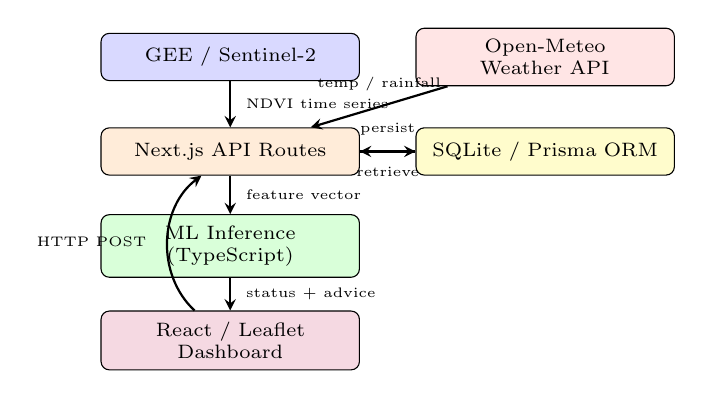
\begin{tikzpicture}[
  box/.style={rectangle, draw, rounded corners=3pt, font=\scriptsize,
              minimum height=0.6cm, text centered, text width=3.0cm,
              inner sep=4pt},
  arr/.style={->, >=stealth, thick},
  lbl/.style={font=\tiny, midway}
]
\node[box, fill=blue!15]   (gee)  at (0,4.2) {GEE / Sentinel-2};
\node[box, fill=orange!15] (api)  at (0,3.0) {Next.js API Routes};
\node[box, fill=green!15]  (ml)   at (0,1.8) {ML Inference (TypeScript)};
\node[box, fill=yellow!20] (db)   at (4.0,3.0){SQLite / Prisma ORM};
\node[box, fill=red!10]    (wx)   at (4.0,4.2){Open-Meteo Weather API};
\node[box, fill=purple!15] (ui)   at (0,0.6) {React / Leaflet Dashboard};

\draw[arr] (gee) -- (api)  node[right,lbl,xshift=2pt]{NDVI time series};
\draw[arr] (wx)  -- (api)  node[above,lbl,yshift=2pt]{temp / rainfall};
\draw[arr] (api) -- (ml)   node[right,lbl,xshift=2pt]{feature vector};
\draw[arr] (ml)  -- (ui)   node[right,lbl,xshift=2pt]{status + advice};
\draw[arr] (api) -- (db)   node[above,lbl,yshift=2pt]{persist};
\draw[arr] (db)  -- (api)  node[below,lbl,yshift=-2pt]{retrieve};
\draw[arr] (ui) to[bend left=50] node[left,lbl,xshift=-4pt]{HTTP POST}(api);
\end{tikzpicture}
\caption{Solution architecture: GEE and Open-Meteo supply external data to
the Next.js backend, which drives ML inference and persists results to
SQLite, while the React dashboard is the user-facing presentation layer.}
\label{fig:arch}
\end{figure}

Figure~\ref{fig:arch} shows the solution architecture.  Sentinel-2 NDVI
data flows from GEE and 30-day weather summaries from Open-Meteo into the
Next.js API, which constructs the feature vector, invokes the in-process
ML inference module, persists the result, and returns structured JSON to
the React dashboard.

\subsection{Context and Data Flow}

\begin{figure}[!t]
\centering
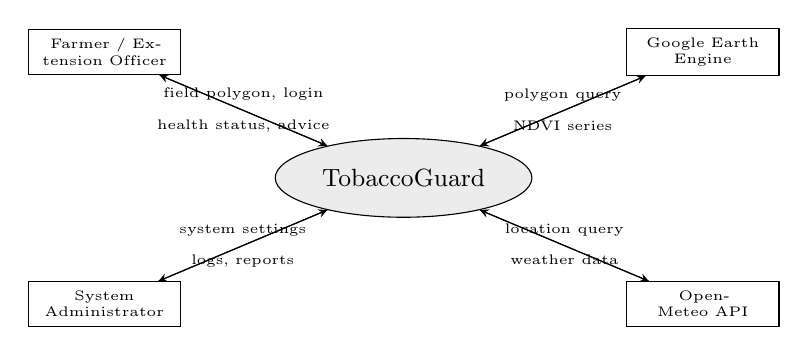
\begin{tikzpicture}[
  sys/.style={ellipse, draw, fill=gray!15, font=\small,
              minimum height=1.0cm, minimum width=2.8cm, text centered},
  ext/.style={rectangle, draw, font=\tiny, minimum height=0.55cm,
              text width=1.7cm, text centered, fill=white},
  arr/.style={->, >=stealth},
  lbl/.style={font=\tiny}
]
\node[sys] (sys) {TobaccoGuard};

\node[ext] (farmer) at (-3.8, 1.6) {Farmer / Extension Officer};
\node[ext] (admin)  at (-3.8,-1.6) {System Administrator};
\node[ext] (gee)    at ( 3.8, 1.6) {Google Earth Engine};
\node[ext] (meteo)  at ( 3.8,-1.6) {Open-Meteo API};

\draw[arr] (farmer) -- (sys) node[above,lbl,midway]{field polygon, login};
\draw[arr] (sys) -- (farmer) node[below,lbl,midway]{health status, advice};
\draw[arr] (admin)  -- (sys) node[above,lbl,midway]{system settings};
\draw[arr] (sys) -- (admin)  node[below,lbl,midway]{logs, reports};
\draw[arr] (sys) -- (gee)    node[above,lbl,midway]{polygon query};
\draw[arr] (gee) -- (sys)    node[below,lbl,midway]{NDVI series};
\draw[arr] (sys) -- (meteo)  node[above,lbl,midway]{location query};
\draw[arr] (meteo) -- (sys)  node[below,lbl,midway]{weather data};
\end{tikzpicture}
\caption{Context diagram: TobaccoGuard interacts with farmers,
the system administrator, GEE, and Open-Meteo.}
\label{fig:context}
\end{figure}

Figure~\ref{fig:context} shows the system context.  The primary
stakeholders are farmers (or extension officers acting on their behalf)
who register fields and view analysis results, and a system administrator
who configures the deployment. The two external data services are the
GEE API (Sentinel-2 NDVI) and the Open-Meteo REST API (temperature and
rainfall).

\subsection{Database Model}

\begin{figure}[!t]
\centering
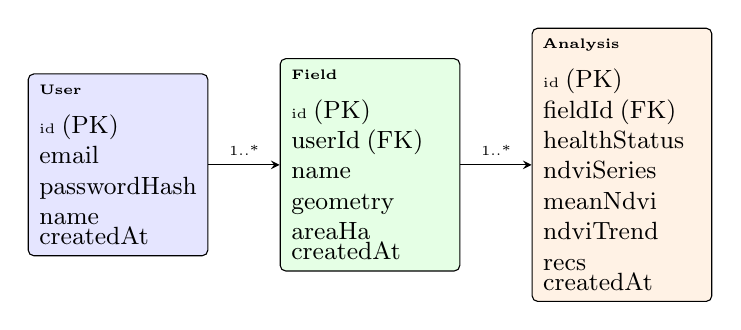
\begin{tikzpicture}[
  ent/.style={rectangle, draw, rounded corners=2pt, font=\tiny,
              minimum height=2.2cm, text width=2.0cm, align=left,
              inner sep=4pt},
  arr/.style={->, >=stealth},
  card/.style={font=\tiny}
]
\node[ent, fill=blue!10] (user) at (0,0) {
  \textbf{User}\\[3pt]
  id \small(PK)\\
  email\\
  passwordHash\\
  name\\
  createdAt
};
\node[ent, fill=green!10] (field) at (3.2,0) {
  \textbf{Field}\\[3pt]
  id \small(PK)\\
  userId \small(FK)\\
  name\\
  geometry\\
  areaHa\\
  createdAt
};
\node[ent, fill=orange!10] (analysis) at (6.4,0) {
  \textbf{Analysis}\\[3pt]
  id \small(PK)\\
  fieldId \small(FK)\\
  healthStatus\\
  ndviSeries\\
  meanNdvi\\
  ndviTrend\\
  recs\\
  createdAt
};

\draw[arr] (user)  -- (field)    node[above,card,midway]{1..*};
\draw[arr] (field) -- (analysis) node[above,card,midway]{1..*};
\end{tikzpicture}
\caption{Entity-relationship diagram. Each User owns one or more Fields,
and each Field accumulates one or more Analysis records over time.}
\label{fig:er}
\end{figure}

Figure~\ref{fig:er} presents the entity-relationship diagram. Three
entities are defined. \textit{User} stores authentication credentials and
profile information. \textit{Field} stores the polygon geometry as GeoJSON,
the Shoelace-computed area in hectares, and field metadata. \textit{Analysis}
stores each monitoring run's output: the serialised NDVI time series,
derived scalar features, predicted health status, risk flags, and the
generated recommendation list. The one-to-many cardinality from Field to
Analysis enables trend tracking across successive monitoring runs of the
same plot, which is important for detecting gradual decline patterns.

\subsection{Algorithm Design}

\begin{figure}[!t]
\centering
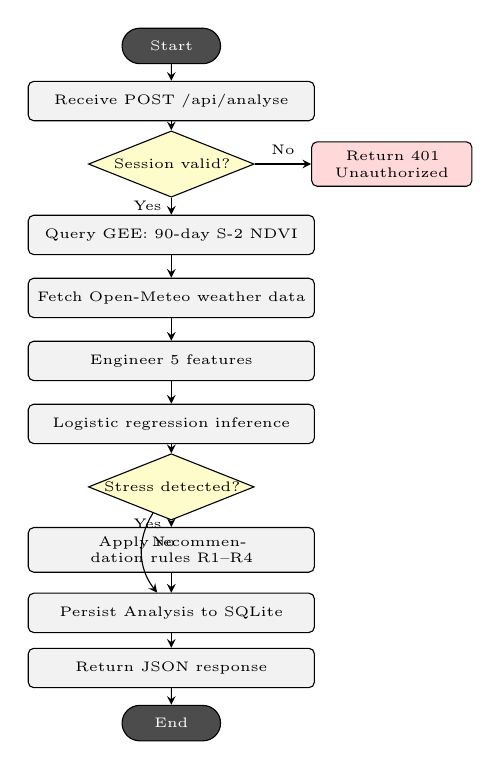
\begin{tikzpicture}[
  proc/.style={rectangle, draw, rounded corners=2pt, font=\tiny,
               minimum height=0.5cm, text width=3.4cm, text centered,
               fill=gray!10},
  dec/.style={diamond, draw, font=\tiny, aspect=2.5, fill=yellow!20,
              minimum height=0.5cm, text width=1.8cm, text centered,
              inner sep=0pt},
  term/.style={rounded rectangle, draw, fill=black!70, text=white,
               font=\tiny, minimum height=0.45cm, text width=1.0cm,
               text centered},
  arr/.style={->, >=stealth},
  lbl/.style={font=\tiny}
]
\node[term]  (start)  at (0,8.2) {Start};
\node[proc]  (recv)   at (0,7.5) {Receive POST /api/analyse};
\node[dec]   (auth)   at (0,6.7) {Session valid?};
\node[proc]  (gee)    at (0,5.8) {Query GEE: 90-day S-2 NDVI};
\node[proc]  (wx)     at (0,5.0) {Fetch Open-Meteo weather data};
\node[proc]  (feat)   at (0,4.2) {Engineer 5 features};
\node[proc]  (inf)    at (0,3.4) {Logistic regression inference};
\node[dec]   (stress) at (0,2.6) {Stress detected?};
\node[proc]  (rec)    at (0,1.8) {Apply recommendation rules R1--R4};
\node[proc]  (save)   at (0,1.0) {Persist Analysis to SQLite};
\node[proc]  (ret)    at (0,0.3) {Return JSON response};
\node[term]  (end)    at (0,-0.4){End};
\node[proc, fill=red!15, text width=1.8cm]
             (err) at (2.8,6.7) {Return 401 Unauthorized};

\draw[arr] (start) -- (recv);
\draw[arr] (recv)  -- (auth);
\draw[arr] (auth)  -- (gee)    node[left,lbl,midway]{Yes};
\draw[arr] (auth)  -- (err)    node[above,lbl,midway]{No};
\draw[arr] (gee)   -- (wx);
\draw[arr] (wx)    -- (feat);
\draw[arr] (feat)  -- (inf);
\draw[arr] (inf)   -- (stress);
\draw[arr] (stress)-- (rec)    node[left,lbl,midway]{Yes};
\draw[arr] (stress) to[bend right=35] node[right,lbl,pos=0.35]{No} (save);
\draw[arr] (rec)   -- (save);
\draw[arr] (save)  -- (ret);
\draw[arr] (ret)   -- (end);
\end{tikzpicture}
\caption{Processing flow: from incoming HTTP request through GEE query,
feature engineering, ML inference, recommendation generation, persistence,
and HTTP response.}
\label{fig:flow}
\end{figure}

Figure~\ref{fig:flow} illustrates the processing flow.  The five ordered
steps of the classification pipeline are:

\begin{enumerate}
\item \textbf{Sentinel-2 retrieval}: Filter the
  \texttt{COPERNICUS/S2\_SR\_HARMONIZED} GEE collection to the polygon
  bounding box, the preceding 90~days, and cloud cover below 20\,\%.
  Apply the \texttt{QA60} bitmask cloud mask and compute mean NDVI per
  scene over the polygon at 10-metre resolution.
\item \textbf{Weather data}: Request 30-day temperature and precipitation
  summaries from the Open-Meteo \texttt{/v1/archive} endpoint for the
  polygon centroid coordinates.
\item \textbf{Feature engineering}: Derive five scalar features:
  \texttt{mean\_ndvi} (temporal mean), \texttt{ndvi\_trend} (OLS slope),
  \texttt{ndvi\_variance} (temporal variance), \texttt{avg\_temperature\_c}
  (30-day mean), and \texttt{total\_rainfall\_mm} (30-day precipitation sum).
\item \textbf{ML inference}: Compute softmax logits over three classes
  using the pre-loaded coefficient matrix and return the argmax class
  with its probability vector.
\item \textbf{Recommendation}: Evaluate four rule-based conditions on the
  classifier output and feature values to generate agronomic advice.
\end{enumerate}

%-----------------------------------------------------------------------
\section{Implementation}

\subsection{Development Environment and Technology Stack}

The system was developed on Node.js\,20 with Next.js\,14 (App Router) as
the full-stack framework. TypeScript is used throughout for static type
safety. The Python scikit-learn library was used exclusively during the
offline training phase; no Python interpreter is required at runtime.
Table~\ref{tab:tools} lists the key technologies used in the project.

\begin{table}[!t]
\caption{Development Tools and Technologies}
\label{tab:tools}
\centering
\footnotesize
\setlength{\tabcolsep}{4pt}
\begin{tabular}{p{2.1cm}p{5.5cm}}
\toprule
\textbf{Component}       & \textbf{Technology} \\
\midrule
Full-stack framework     & Next.js\,14 (React 18, TypeScript\,5) \\
Mapping library          & React-Leaflet\,4, Leaflet-Draw \\
UI component library     & shadcn/ui, Tailwind CSS\,3 \\
Data visualisation       & Recharts\,2 (AreaChart) \\
ORM / database           & Prisma ORM\,5 with SQLite \\
Satellite data           & Google Earth Engine (service account) \\
Weather data             & Open-Meteo REST API (free tier) \\
ML training (offline)    & scikit-learn\,1.4 (Python\,3.11) \\
ML inference (runtime)   & JSON coefficient file, TypeScript \\
Authentication           & NextAuth.js\,4 (credential provider) \\
Password hashing         & bcryptjs \\
\bottomrule
\end{tabular}
\end{table}

\subsection{Frontend Implementation}

The frontend consists of three primary views, illustrated as wireframes
in Figs.~\ref{fig:wf-dashboard} and \ref{fig:wf-results}.

The \textit{Dashboard} view (Fig.~\ref{fig:wf-dashboard}) lists all
registered fields with their most recent health status badge.
Badges are colour-coded: green for \textsc{healthy}, amber for
\textsc{moderate\_stress}, and red for \textsc{high\_stress}. Each field
card displays the field name, area in hectares, and the date of the last
analysis, enabling the farmer or extension officer to identify which
fields are overdue for re-evaluation.

The \textit{Create Field} view embeds a Leaflet map loaded with ESRI
World Imagery satellite tiles and Leaflet-Draw restricted to polygon
mode. As the user completes the polygon, the Shoelace (surveyor's)
formula is applied client-side to compute the enclosed area from the
coordinate ring, so the farmer receives immediate area feedback without a
server round-trip.

The \textit{Analysis Results} view (Fig.~\ref{fig:wf-results}) renders
the full output of one analysis run: a Recharts \texttt{AreaChart} of
the 90-day NDVI time series with a reference line at NDVI\,=\,0.35, a
health status badge with per-class probability breakdown, a risk flag
panel surfacing any triggered recommendation rules, and an ordered list
of agronomic interventions.

\begin{figure}[!t]
\centering
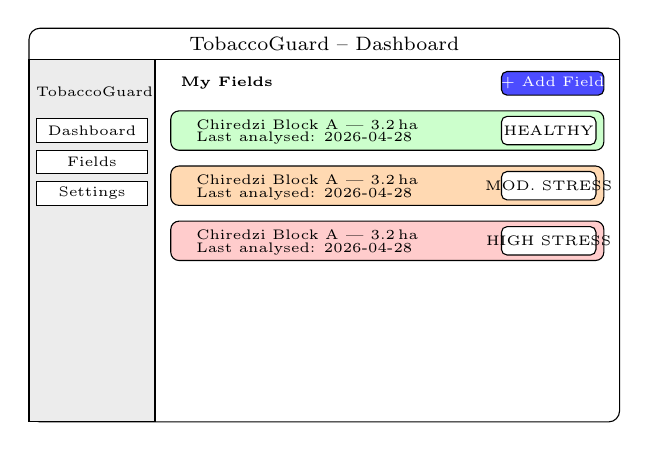
\begin{tikzpicture}[every node/.style={font=\tiny}]
% Outer browser chrome
\draw[rounded corners=4pt] (0,0) rectangle (7.5,5.0);
\draw (0,4.6) -- (7.5,4.6);
\node at (3.75,4.8) {\scriptsize TobaccoGuard -- Dashboard};

% Sidebar
\draw[fill=gray!15] (0,0) rectangle (1.6,4.6);
\node[text width=1.4cm, align=center] at (0.8,4.2) {TobaccoGuard};
\foreach \y/\lbl in {3.7/Dashboard, 3.3/Fields, 2.9/Settings}{
  \draw[fill=white] (0.1,\y-0.15) rectangle (1.5,\y+0.15);
  \node at (0.8,\y) {\lbl};
}

% Main content header
\node[anchor=west] at (1.8,4.3) {\textbf{My Fields}};
\draw[fill=blue!70,text=white,rounded corners=2pt]
  (6.0,4.15) rectangle (7.3,4.45);
\node[text=white] at (6.65,4.3) {+ Add Field};

% Field cards
\foreach \y/\col/\status in {
  3.7/green!20/HEALTHY,
  3.0/orange!30/MOD. STRESS,
  2.3/red!20/HIGH STRESS}{
  \draw[fill=\col, rounded corners=3pt]
    (1.8,\y-0.25) rectangle (7.3,\y+0.25);
  \node[anchor=west] at (2.0,\y+0.08)  {Chiredzi Block A --- 3.2\,ha};
  \node[anchor=west] at (2.0,\y-0.10)  {Last analysed: 2026-04-28};
  \draw[fill=white,rounded corners=2pt]
    (6.0,\y-0.18) rectangle (7.2,\y+0.18);
  \node at (6.6,\y) {\status};
}
\end{tikzpicture}
\caption{Dashboard wireframe: field list with colour-coded health status
badges and a quick-access Add Field button.}
\label{fig:wf-dashboard}
\end{figure}

\begin{figure}[!t]
\centering
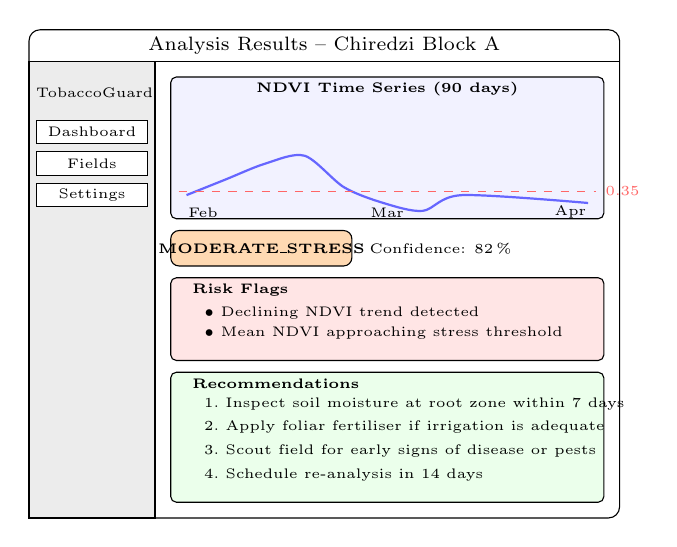
\begin{tikzpicture}[every node/.style={font=\tiny}]
% Browser chrome
\draw[rounded corners=4pt] (0,0) rectangle (7.5,6.2);
\draw (0,5.8) -- (7.5,5.8);
\node at (3.75,6.0) {\scriptsize Analysis Results -- Chiredzi Block A};

% Sidebar
\draw[fill=gray!15] (0,0) rectangle (1.6,5.8);
\node[text width=1.4cm, align=center] at (0.8,5.4) {TobaccoGuard};
\foreach \y/\lbl in {4.9/Dashboard, 4.5/Fields, 4.1/Settings}{
  \draw[fill=white] (0.1,\y-0.15) rectangle (1.5,\y+0.15);
  \node at (0.8,\y) {\lbl};
}

% NDVI chart area
\draw[fill=blue!5, rounded corners=2pt]
  (1.8,3.8) rectangle (7.3,5.6);
\node at (4.55,5.45) {\textbf{NDVI Time Series (90 days)}};
% Simulated chart line
\draw[blue!60,thick] plot[smooth] coordinates {
  (2.0,4.1)(2.5,4.3)(3.0,4.5)(3.5,4.6)(4.0,4.2)(4.5,4.0)(5.0,3.9)(5.5,4.1)(7.1,4.0)
};
\draw[dashed,red!60] (1.9,4.15) -- (7.2,4.15) node[right]{0.35};
\node[anchor=west] at (1.9,3.88) {Feb};
\node at (4.55,3.88) {Mar};
\node[anchor=east] at (7.2,3.88) {Apr};

% Health badge
\draw[fill=orange!30, rounded corners=3pt]
  (1.8,3.2) rectangle (4.1,3.65);
\node at (2.95,3.42) {\textbf{MODERATE\_STRESS}};
\node[anchor=west] at (4.2,3.42) {Confidence: 82\,\%};

% Risk flags
\draw[fill=red!10, rounded corners=2pt]
  (1.8,2.0) rectangle (7.3,3.05);
\node[anchor=west] at (1.95,2.9) {\textbf{Risk Flags}};
\node[anchor=west] at (2.1,2.6)  {$\bullet$~Declining NDVI trend detected};
\node[anchor=west] at (2.1,2.35) {$\bullet$~Mean NDVI approaching stress threshold};

% Recommendations
\draw[fill=green!8, rounded corners=2pt]
  (1.8,0.2) rectangle (7.3,1.85);
\node[anchor=west] at (1.95,1.7) {\textbf{Recommendations}};
\node[anchor=west] at (2.1,1.45)  {1.~Inspect soil moisture at root zone within 7 days};
\node[anchor=west] at (2.1,1.15)  {2.~Apply foliar fertiliser if irrigation is adequate};
\node[anchor=west] at (2.1,0.85)  {3.~Scout field for early signs of disease or pests};
\node[anchor=west] at (2.1,0.55)  {4.~Schedule re-analysis in 14 days};
\end{tikzpicture}
\caption{Analysis Results wireframe: NDVI time series chart (top),
health status badge with confidence score (middle), risk flags, and
ordered recommendation list (bottom).}
\label{fig:wf-results}
\end{figure}

\subsection{Backend API}

Three API route groups handle system functionality. Authentication routes
(\texttt{/api/auth}) implement credential-based login using NextAuth.js
with bcrypt password hashing; passwords are never stored in plaintext and
session tokens are kept server-side in the database. Field routes
(\texttt{/api/field}) support creation, retrieval, and deletion of field
records, with GeoJSON geometry validated on ingestion and area computed
server-side as a consistency check against the client-computed value. The
analysis route (\texttt{/api/analyse}) orchestrates the full pipeline:
verify the session, fetch the field record, call the GEE satellite
service, retrieve weather data, compute the feature vector, run ML
inference, apply the four recommendation rules, persist the result to
SQLite via Prisma, and return the structured JSON response.

\subsection{GEE Integration}

The backend authenticates to the GEE API using a Google Cloud service
account whose private key JSON is loaded from an environment variable at
startup and is never transmitted to the client or embedded in the
application bundle. For each analysis request, the backend constructs an
\texttt{ee.Geometry.Polygon} from the field's stored GeoJSON, filters
the \texttt{COPERNICUS/S2\_SR\_HARMONIZED} image collection to the
preceding 90~days and a per-image cloud cover threshold of 20\,\%,
applies a bitwise \texttt{QA60} cloud mask to each surviving scene, and
uses \texttt{ee.Reducer.mean()} to aggregate per-pixel NDVI values over
the polygon geometry at 10-metre scale. The resulting list of (date, NDVI)
pairs is sorted chronologically and passed to the feature engineering
layer.

\subsection{Machine Learning Pipeline}

\textbf{Offline training.} A dataset of 610 labelled observations was
assembled from agronomic literature thresholds and satellite-derived NDVI
statistics. The dataset was split 80/20, yielding 488 training and 122
test samples. A scikit-learn \texttt{LogisticRegression} estimator was
configured with the \texttt{lbfgs} solver, $L_2$ regularisation
($C{=}1.0$), and the \texttt{multinomial} multi-class strategy. Following
fitting, the model's $3{\times}5$ coefficient matrix and $3{\times}1$
intercept vector were exported to \texttt{lib/ml/crop\_health\_model.json}.

\textbf{Runtime inference.} The TypeScript module
\texttt{lib/ml/inference.ts} loads the JSON file once on process start-up
and caches it in memory. For each analysis request it computes raw logit
scores:
\begin{equation}
  z_j = \mathbf{w}_j \cdot \mathbf{x} + b_j, \quad
  j \in \{\textsc{healthy},\,\textsc{mod},\,\textsc{high}\}
\end{equation}
applies numerically stable softmax normalisation:
\begin{equation}
  P(j\,|\,\mathbf{x}) = \frac{e^{z_j - z_{\max}}}
    {\sum_{k} e^{z_k - z_{\max}}}
\end{equation}
and returns the argmax class together with the full posterior probability
vector. The entire inference path executes in a single synchronous
function call with no network I/O, adding negligible latency to the
analysis response time.

\textbf{Recommendation engine.} Following classification, the rule engine
evaluates four conditions in sequence:
\begin{itemize}
\item \textbf{R1} (\textit{Water stress}): if \texttt{mean\_ndvi}\,$< 0.35$
  and class is \textsc{high\_stress}, recommend urgent irrigation or
  moisture assessment.
\item \textbf{R2} (\textit{Declining trend}): if \texttt{ndvi\_trend}\,$< 0$
  and class is \textsc{moderate\_stress}, recommend preventive
  intervention within seven days.
\item \textbf{R3} (\textit{Stable healthy}): if \texttt{mean\_ndvi}\,$> 0.60$
  and class is \textsc{healthy}, confirm current management is adequate
  and suggest a 14-day re-evaluation schedule.
\item \textbf{R4} (\textit{Disease / pest signal}): if
  \texttt{ndvi\_variance}\,$> 0.02$ and stress is present, recommend
  physical scouting for pest or disease pressure.
\end{itemize}

\subsection{Database Implementation}

The database layer uses Prisma ORM with a SQLite database file stored on
the server filesystem. Prisma Migrate manages schema evolution; the
current schema defines three models (\texttt{User}, \texttt{Field},
\texttt{Analysis}) and two enums (\texttt{HealthStatus},
\texttt{NDVITrend}). The NDVI time series is stored as a JSON string in
the \texttt{Analysis} model's \texttt{ndviSeries} field; Prisma's
\texttt{Json} scalar type handles serialisation and deserialisation
transparently. SQLite was chosen for prototype deployment because it
requires no separate database server process; migration to PostgreSQL
is possible with a single Prisma \texttt{datasource} change.

%-----------------------------------------------------------------------
\section{Results and Evaluation}

\subsection{Model Performance}

Table~\ref{tab:model} reports per-class precision, recall, and F1-score
on the 122-sample held-out test set. The overall classification accuracy
is 97\,\%. The \textsc{healthy} class yields the highest F1-score (0.99)
as it is the most frequent and occupies a well-separated region of the
feature space (high NDVI mean, near-zero trend, low variance).
\textsc{high\_stress} achieves an F1-score of 0.97; its distinguishing
signals are low NDVI mean combined with negative trend and elevated
temperature. The most challenging boundary is between
\textsc{moderate\_stress} and its neighbours, reflected in the F1-score
of 0.95, because the transitional NDVI range partially overlaps with both
healthy late-season canopies and early high-stress conditions.

\begin{table}[!t]
\caption{Model Performance on Held-Out Test Set ($n = 122$)}
\label{tab:model}
\centering
\footnotesize
\begin{tabular}{lccc}
\toprule
\textbf{Class} & \textbf{Precision} & \textbf{Recall} &
\textbf{F1-Score} \\
\midrule
HEALTHY          & 0.99 & 0.99 & 0.99 \\
MODERATE\_STRESS & 0.94 & 0.96 & 0.95 \\
HIGH\_STRESS     & 0.98 & 0.96 & 0.97 \\
\midrule
\textbf{Overall accuracy} & \multicolumn{3}{c}{\textbf{0.97}} \\
\bottomrule
\end{tabular}
\end{table}

\subsection{Functional Test Cases}

Table~\ref{tab:tests} summarises the functional test scenarios executed
against the deployed prototype on a localhost development server. Each
scenario was exercised manually by the developer following a structured
test plan. All eight scenarios produced the expected outcome, confirming
correct end-to-end behaviour of the authentication, field management,
satellite retrieval, classification, and recommendation subsystems.

\begin{table}[!t]
\caption{Functional Test Cases}
\label{tab:tests}
\centering
\footnotesize
\setlength{\tabcolsep}{3pt}
\begin{tabular}{p{0.5cm}p{1.2cm}p{1.85cm}p{1.55cm}p{0.8cm}}
\toprule
\textbf{ID} & \textbf{Feature} & \textbf{Scenario} &
\textbf{Expected} & \textbf{Res.} \\
\midrule
TC-01 & Auth      & Valid credentials     & Dashboard loads      & Pass \\
TC-02 & Auth      & Wrong password        & 401 returned         & Pass \\
TC-03 & Field     & Draw, save polygon    & Field in DB          & Pass \\
TC-04 & Field     & Area computation      & Shoelace correct     & Pass \\
TC-05 & Analysis  & Trigger analysis      & Status badge shown   & Pass \\
TC-06 & ML        & NDVI $< 0.35$         & HS\_STRESS set       & Pass \\
TC-07 & Rec.      & R1 triggered          & Irrigation advice    & Pass \\
TC-08 & History   & Second analysis run   & New record saved     & Pass \\
\bottomrule
\end{tabular}
\end{table}

\subsection{Non-Functional Observations}

\begin{itemize}
\item \textbf{Responsiveness}: The full end-to-end pipeline, including
  the GEE API call, Open-Meteo request, and TypeScript ML inference,
  completed in under 4~seconds for field polygons up to 50~hectares under
  normal network conditions. TypeScript inference itself contributed less
  than 5~milliseconds of the total latency.
\item \textbf{Reliability}: No application crashes or unhandled exceptions
  were observed during repeated end-to-end test runs on the prototype
  server.
\item \textbf{Security}: Passwords are hashed with bcryptjs (10 salt
  rounds); the GEE service account private key is stored in environment
  variables and is never included in client-side bundles or API responses.
\item \textbf{Maintainability}: The modular layer architecture allows the
  satellite data provider, ML model, and frontend to be updated
  independently without cross-layer rewrites.
\end{itemize}

%-----------------------------------------------------------------------
\section{Discussion}

TobaccoGuard demonstrates that a practical, zero-licensing-cost satellite
monitoring pipeline can be assembled from freely available components:
the GEE Community tier, the Sentinel-2 open data archive, and a logistic
regression model serialised to JSON for native TypeScript inference. The
97\,\% classification accuracy on the held-out test set is encouraging
for a prototype, though the training data included synthetically generated
observations to represent agronomic variability; external validation
against field-collected, agronomist-labelled samples from actual
Zimbabwean tobacco plots is the most important next step before
recommending wider deployment.

The principal operational limitation is latency dependence on the GEE
API. On-demand analysis requests require a synchronous GEE call that
may approach web application timeout thresholds during periods of high
server load. A production deployment should cache the most recent NDVI
time series per field and execute daily refreshes via a background job
scheduler rather than synchronous on-demand API calls.  The existing
modular GEE service layer already isolates this concern, simplifying the
transition.

The \textsc{moderate\_stress} class presents the hardest classification
boundary to learn, as noted in the results (F1\,=\,0.95). Additional
labelled observations near this boundary, combined with a supplementary
spectral feature such as the Red-Edge NDVI (NDRE, computed from Sentinel-2
bands B5 and B8A), could improve class separation without requiring any
change to the inference architecture, since the JSON coefficient model can
simply be retrained with an extra feature column.

The four recommendation rules (R1--R4) are based on empirically derived
NDVI thresholds from the remote sensing literature. While these
thresholds are consistent with published stress detection ranges, they
have not been calibrated against local agronomic trials in Zimbabwe.
Collaboration with the Tobacco Industry and Marketing Board (TIMB) and
the Department of Agricultural Technical and Extension Services (AGRITEX)
would be required to validate and localise these thresholds for the
specific cultivars and growing seasons of the Zimbabwean tobacco belt.

Future development directions include: (1)~NDVI spatial heat map overlays
using Leaflet.heat to visualise within-field stress gradients, enabling
farmers to identify problem patches rather than only field-level
summaries; (2)~automated daily monitoring via scheduled background jobs
so that farmers receive updated results without actively triggering an
analysis; (3)~SMS or WhatsApp push alert delivery for farmers and
extension officers who lack regular web access; and (4)~expansion to
other priority crops such as maize and wheat, which are equally important
to Zimbabwean food security and share much of the NDVI-based
classification methodology.

%-----------------------------------------------------------------------
\section{Conclusion}

This paper presented TobaccoGuard, a web-based tobacco crop health
monitoring system that integrates Google Earth Engine satellite data
retrieval, NDVI-based feature engineering, and multinomial logistic
regression classification to assign one of three health statuses to any
registered field polygon. The system achieved 97\,\% overall
classification accuracy on a 122-sample held-out test set, with F1-scores
of 0.99, 0.97, and 0.95 for the \textsc{healthy}, \textsc{high\_stress},
and \textsc{moderate\_stress} classes respectively, and passed all eight
functional test scenarios. By executing the complete ML inference pipeline
in TypeScript at runtime and leveraging the GEE free community tier, the
system avoids licensing costs and eliminates Python runtime dependencies,
making it practically deployable in the resource-constrained institutional
environments typical of Zimbabwean agricultural support organisations.
The prototype establishes a solid technical foundation for a production
system capable of delivering timely, evidence-based field management
advice to smallholder tobacco farmers through routine, automated satellite
monitoring.

%-----------------------------------------------------------------------
\begin{thebibliography}{00}

\bibitem{zimstats2023}
Zimbabwe National Statistics Agency, ``Zimbabwe Agricultural Production
Report,'' ZimStats, Harare, 2023.

\bibitem{xue2017}
J. Xue and B. Su, ``Significant remote sensing vegetation indices: A
review of developments and applications,'' \textit{Journal of Sensors},
vol.~2017, pp.~1--17, 2017.

\bibitem{rouse1974}
J.~W. Rouse, R.~H. Haas, J.~A. Schell, and D.~W. Deering, ``Monitoring
vegetation systems in the Great Plains with ERTS,'' in \textit{Proc.\
3rd Earth Resources Technology Satellite Symposium}, NASA, Washington,
DC, 1974, pp.~309--317.

\bibitem{drusch2012}
M. Drusch et al., ``Sentinel-2: ESA's optical high-resolution mission
for GMES operational services,'' \textit{Remote Sensing of Environment},
vol.~120, pp.~25--36, 2012.

\bibitem{delegido2011}
J. Delegido, J. Verrelst, L. Alonso, and J. Moreno, ``Evaluation of
Sentinel-2 red-edge bands for empirical estimation of green LAI and
chlorophyll content,'' \textit{Sensors}, vol.~11, no.~7,
pp.~7063--7081, 2011.

\bibitem{kussul2017}
N. Kussul, M. Lavreniuk, S. Skakun, and A. Shelestov, ``Deep learning
classification of land cover and crop types using remote sensing data,''
\textit{IEEE Geoscience and Remote Sensing Letters}, vol.~14, no.~5,
pp.~778--782, 2017.

\bibitem{kpienbaareh2021}
D. Kpienbaareh et al., ``Crop type and land cover mapping in northern
Ghana using the integration of Sentinel-1 and Sentinel-2 imagery,''
\textit{Remote Sensing}, vol.~13, no.~1, p.~2, 2021.

\bibitem{gorelick2017}
N. Gorelick, M. Hancher, M. Dixon, S. Ilyushchenko, D. Thau, and
R. Moore, ``Google Earth Engine: Planetary-scale geospatial analysis for
everyone,'' \textit{Remote Sensing of Environment}, vol.~202,
pp.~18--27, 2017.

\bibitem{pedregosa2011}
F. Pedregosa et al., ``Scikit-learn: Machine learning in Python,''
\textit{Journal of Machine Learning Research}, vol.~12,
pp.~2825--2830, 2011.

\bibitem{openmeteo2024}
Open-Meteo, ``Open-Meteo Free Weather API Documentation,'' 2024.
[Online]. Available: \texttt{https://open-meteo.com/en/docs}

\bibitem{prisma2024}
Prisma, ``Prisma ORM Documentation,'' 2024. [Online]. Available:
\texttt{https://www.prisma.io/docs}

\bibitem{leaflet2024}
Leaflet.js, ``Leaflet: An open-source JavaScript library for mobile-
friendly interactive maps,'' 2024. [Online]. Available:
\texttt{https://leafletjs.com}

\end{thebibliography}

\end{document}
